\documentclass[a4paper,8pt]{article}
\usepackage[utf8x]{inputenc}
\usepackage[margin=0.7in]{geometry}
% \usepackage[top=2in, bottom=1.5in, left=1in, right=1in]{geometry} -->
\usepackage{graphicx}
\usepackage{listings}
%opening
\title{Teoría de Lenguajes\\ \textbf{TP2: “Micro HTML Prettyprint - segunda parte”}}
\author{1º Cuatrimestre 2013} 
\date{}


\begin{document}

\maketitle

\begin{center}
\vspace{10cm}

\begin{tabular}{|c|c|}
\hline
\hline
\textbf{Nombre}&\textbf{email}\\
\hline
\hline
Pablo Herrero (LU:332/07)   & pablodherrero@gmail.com   \\
\hline
\hline
\end{tabular}
\end{center}

\newpage

\begin{section}{Introducción}
El Trabajo Práctico consiste en implementar un parser de HTML, el lenguaje de marcado más utilizado hoy en dia para la representación documentos en la World Wide Web.

Los distintos browsers se encargan de mostrar el contenido de las página escritas en HTML de forma tal que sea visualmente actractivo para el usuario.

Para este TP se realizará un procesador que formateará el contenido de una documento HTML, generando un documento nuevo, de manera de que el documento original sea fácilmente legible por cualquiera que comprenda el lenguaje de marcado en cuestion, como se muestra a continuación.

\begin{figure}[h!]
  \centering
  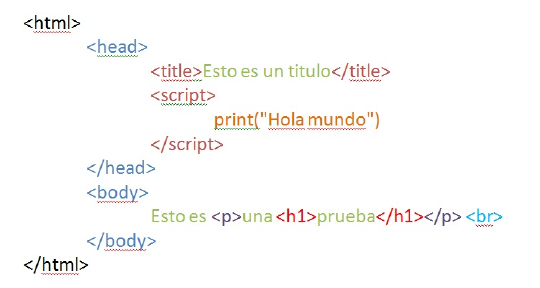
\includegraphics[scale=0.70]{salida.png}
  \caption{\texttt{Salida esperada para el siguiente HTML ``$<html> <head><title>$Esto es un titulo$</title> <!–$ esto es un comentario $–> <script> print($”Hola mundo”$)</script></head> <body>$ Esto es $<p>$una $<h1>$prueba$</h1></p> <br></body></html>$''}}
\end{figure}

El trabajo práctico fue dividido en dos partes, la primera consistió en identificar cuál seria la gramática y los componentes léxicos de nuestro lenguaje y la segunda parte consiste en realizar el parser junto con las reglas semánticas que permitirán generar el HTML resultante.
 


\end{section}
\newpage
\begin{section}{Gramática}
\begin{subsection}{Descripción del HTML reducido a identificar}
Para simplificar el lenguaje, ya que HTML es muy completo y extenso, sólo se considerará un subconjunto de tags válidos, no se permitirán atributos y se espera que todos los tags tengan su tag de cierre correspondiente (salvo $<br>$).\\


Los tags que se considerarán son:

\textbf{$<html>-<head>-<body>-<title>-<script>-<div>-<h1>-<p>-<br>$}.\\

Con las siguiente restricciones:

\begin{itemize}
 \item Es obligatorio que el documento completo esté rodeado por tags de apertura y cierre $<html>$
\item dentro del html puede tener una sección opcional $<head>$ y otra sección también opcional $<body>$. Si hay una sección $<head>$ esta debe encontrarse antes del body.
\item dentro de la sección head pueden aparecer indistintamente y en orden no preestablecido secciones $<title>$ y $<script>$
\item $<title>$ contiene texto sin tags
\item dentro de la sección $<script>$ puede haber cualquier cosa salvo el tag de cierre de dicha sección
\item dentro de la sección $<body>$ tendremos bloques de texto con subsecciones (div, h1 o p) o con tags $<br>$ sueltos, las subsecciones se comportan como la sección $<body>$
\end{itemize}


\end{subsection}

\begin{subsection}{Gramática utilizada para la primera parte del tp}
\bigskip

\begin{verbatim}
S -> E<html>EAE</html>E | E<html>ECE</html>E | E<html>E</html>E
A -> <head>EBE</head>ECE
B -> <title>T</title>EBE | <script>T</script>EBE | lambda
C -> <body>EDE</body> | <body>TDT</body>  | lambda
D -> T D | lambda | <div>EDE</div>EDE | <p>EDE</p> EDE | <h1>EDE</h1> EDE |
    |<br>EDE | <div>TDT</div>TDT | <p>TDT</p>TDT | <h1>TDT</h1>TDT | <br>TDT
E -> espacioE | E<!–-T-–>E  | lambda 
T -> (a|...|z|A|...|Z|0|...|9|...|&|;|espacio|... )T | E |lambda  
espacio pertenece a {“ “}

\end{verbatim}
\bigskip

Descripción de la gramática
\begin{enumerate}
 \item Todas las derivaciones del símbolo distinguido comienzan (terminan) con cero o más espacios y luego un tag de apertura (cierre) de html, la derivación que contiene A corresponde a un HTML con head mientras que la que contiene C es un HTML que no tiene head
 \item La derivación de A corresponde a un head seguido de cero o más espacios, cero o un body y cero o más espacios
\item La derivación de B es el contenido que puede estar dentro de un head, estos son titles (conteniendo texto) o scripts (conteniendo texto), en ambos casos puede haber cero o más ocurrencias
\item La derivación de C permite que haya cero o un body conteniendo tags, ver EDE y TDT en el punto siguiente.
\item Derivaciones de D: a) TD  , esto permite agregar texto a izquierda de los tags, como el tag puede derivar en $\lambda$ esto también permite terminar con texto a derecha “quitando” el último D - b) Las derivaciones rodeades de div, p y h1 permiten generar estos tags, en todos los casos contienen EDE que permite nuevos tags rodeados de cero o más espacios o derivar D a TD y generar texto - c) La derivación $<br>EDE$ permite generar el tag $<br>$ - d) Las derivaciones que contienen TDT son todas redundantes por lo expuesto en 5.a y 5.b pero hacen que los ejemplos sean más compactos
\item Esta derivación permite generar cero o más espacios o comentarios
\item Esta derivación permite generar texto de longitud cero o mayor, se agregan los símbolos $\&$ y $;$ para poder codificar las entidades html y se permite derivar a E para poder incluir comentarios ya que esto siempre es válido
\end{enumerate}

\end{subsection}

\begin{subsection}{Gramática corregida}
En las correcciones se nos indicó que debíamos completar los tokens léxicos para los tags y definir correctamente el conjunto de terminales para el texto.
\bigskip

\begin{verbatim}
S -> E I_HTML EAE F_HTML E | E I_HTML ECE F_HTML E | E I_HTML E F_HTML E
A -> I_HTML EBE F_HTML ECE
B -> I_TITLE T F_TITLE EBE | I_SCRIPT T F_SCRIPT EBE | lambda
C -> I_BODY EDE F_BODY | I_BODY TDT F_BODY  | lambda
D -> T D | lambda | I_DIV EDE F_DIV EDE | I_P EDE F_P EDE | 
     | I_H1 EDE F_H1 EDE | I_BR EDE | I_DIV TDT F_DIV TDT | 
     | I_P TDT F_P TDT | I_H1 TDT F_H1 TDT | I_BR TDT
E -> WS E | E I_COMMENT T F_COMMENT E  | lambda 
T -> WS TEXTO_SIN_TAGS WS T | lambda 

---------------- TOKENS LEXICOS ---------------------------
I_HTML 	:	'<html>' 
F_HTML 	:	'</html>' 

I_HEAD 	:	'<head>'  
F_HEAD 	:	'</head>' 

I_BODY 	:	'<body>' 
F_BODY 	:	'</body>'

I_TITLE:	'<title>'  
F_TITLE:	'</title>' 
	
I_SCRIPT:	'<script>'  
F_SCRIPT:	'</script>' 
	
I_DIV 	:	'<div>' 
F_DIV 	:	'</div>' 
	
I_H1 	:	'<h1>'  
F_H1 	:	'</h1>' 
	
I_P 	:	'<p>'
F_P 	:	'</p>' 

BR 	:	'<br>'

I_COMMENT:	'<!–-'
F_COMMENT:	'-->'

TEXTO_SIN_TAGS 
	:	(~('<' | '>' | '\t' | '\r'| '\n'))* 

WS 
    :   ('\t' | '\r'| '\n') 


\end{verbatim}
\bigskip
\newpage
 \begin{subsubsection}{Arboles de derivación - Ejemplos}
       \begin{figure}[h!]
      \centering
      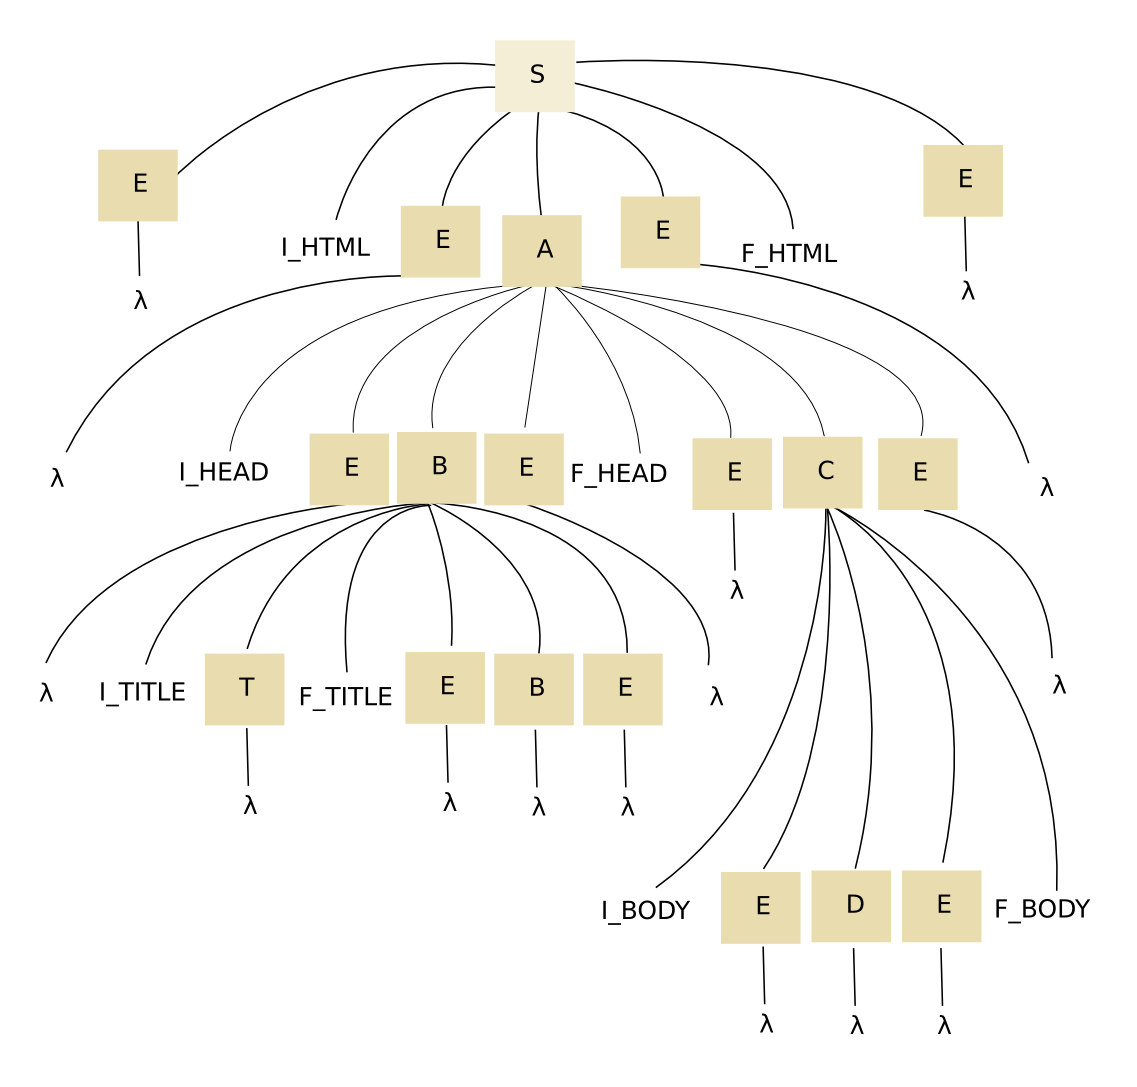
\includegraphics[scale=0.30]{ejemplo1.png}

      \caption{Arbol de derivación para ``$<html><head><title></title></head><body></body></html>$''}
    \end{figure}

    \begin{figure}[h!]
      \centering
      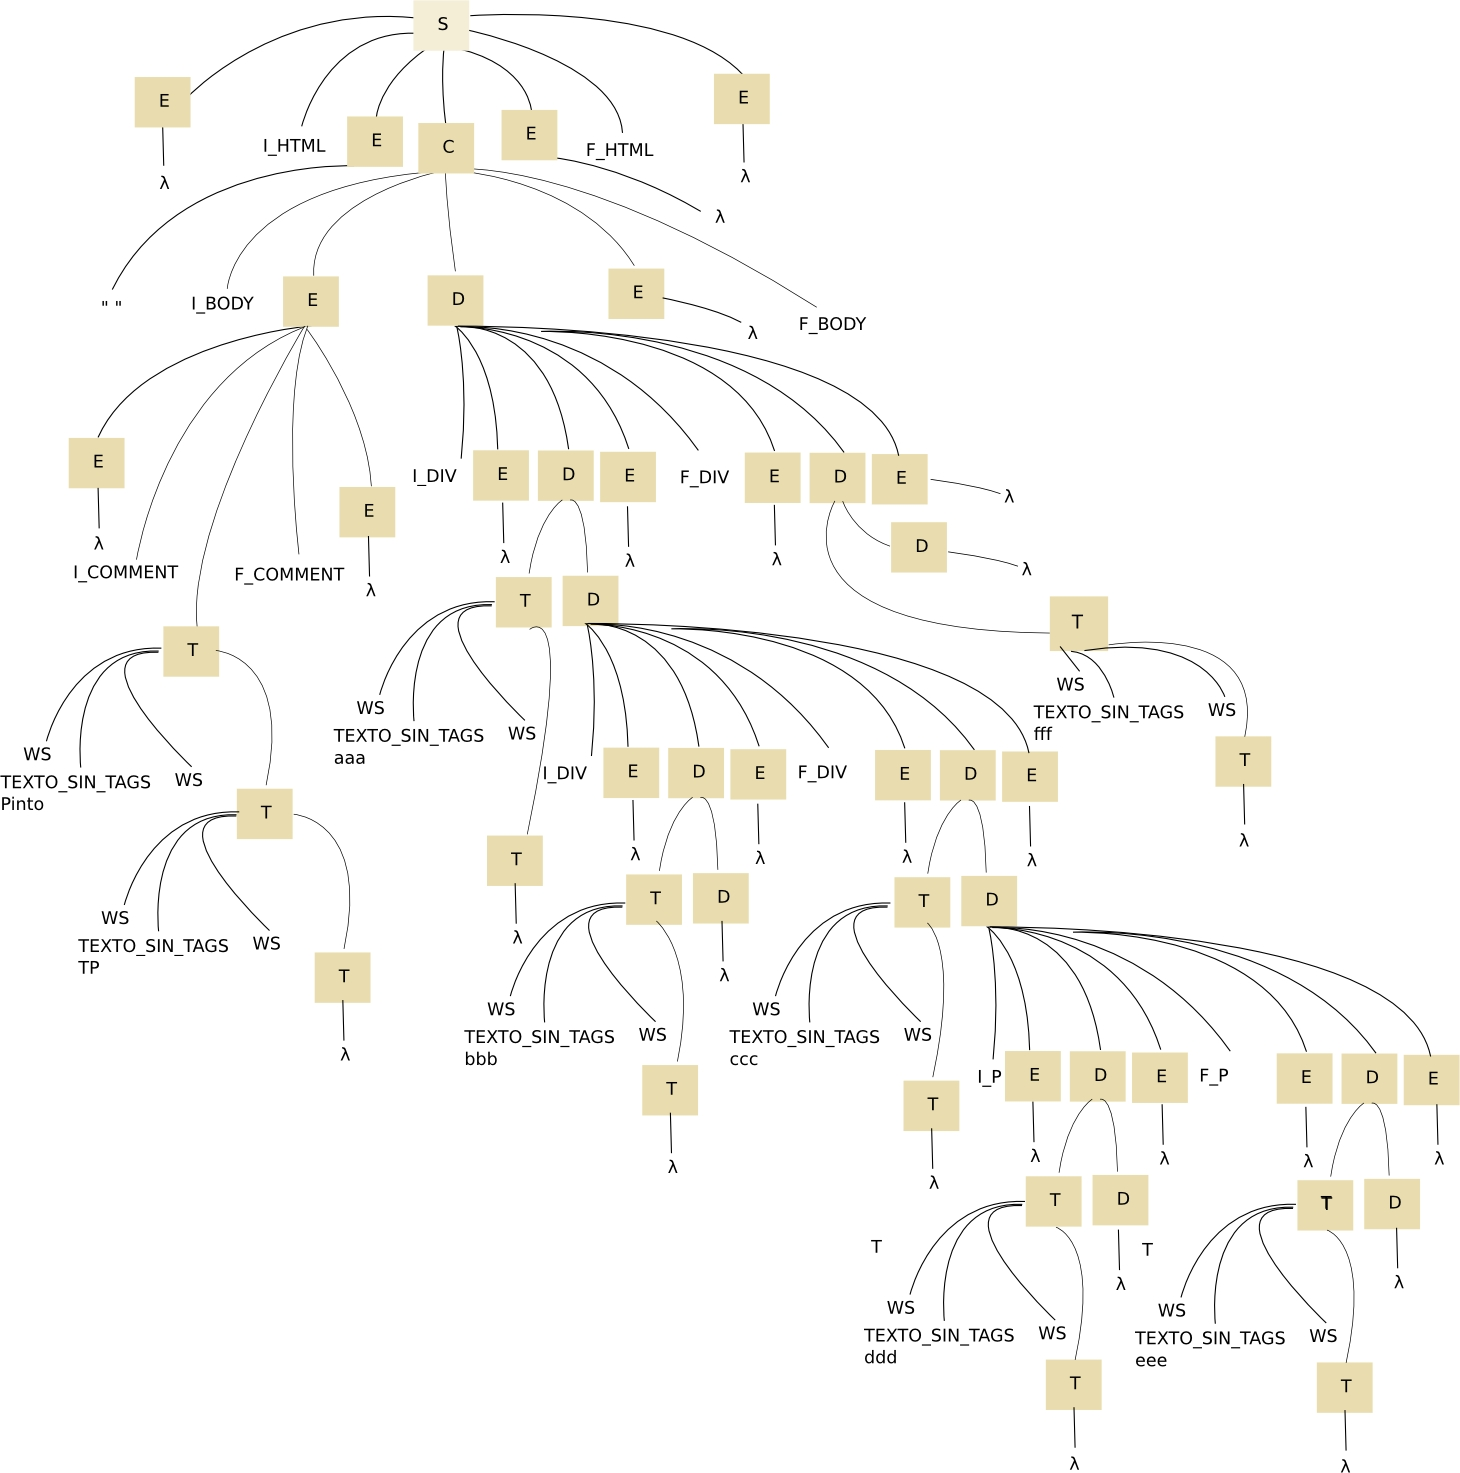
\includegraphics[scale=0.35]{g5188.jpg}

      \caption{Arbol de derivación para ``$<html> <body><!--$ pinto TP $--> <div>aaa<div>bbb</div>ccc<p>ddd</p>eee</div>fff</body></html>$''}
    \end{figure}


 \end{subsubsection}

\end{subsection}
\newpage

\begin{subsection}{Gramática modificada para la segunda parte del tp}

La gramática para la segunda parte fue reescrita desde el comienzo con el fin de ajustarse lo más fielmente posible a las aclaraciones hecha en el enunciado de la 2da parte y permitiendo mayor libertad a la hora de diseñar el lexer y el parser.\\

En esta segunda parte, una vez definida la gramática, se agregarán en la implementación reglas semánticas que permitan:\\
\begin{itemize}
 \item La salida será un documento que se visualice desde un browser como código HTML (Figura 1).
\item El código del HTML de entrada deberá aparecer formateado con cada línea indentada según el nivel de anidación del código del archivo HTML de origen. 
\item A cada clase de token se le deben poder asignar distintos atributos visuales. En cuanto a los atributos visuales, se requiere un color para los tags head y body, otro para los tags title y script, otro para el tag h1, otro para el tag div y otro para el tag br. Otro color para el texto y otro para los scripts.
Se sugiere que cada token quede incluido en un elemento de tipo SPAN que indique de qué clase es.
Por ejemplo:$<SPAN class=``tagH1''>\&lt;h1\&gt;</SPAN>.$

\end{itemize}

A continuacion se copian los Tokens lexicos definidos para esta nueva gramatica y la gramatica LALR utilizada por la implementación:
Notar que en los tokens, los comentarios y espacios en blanco siempre se ignoran y el parser nunca los recibe.
Luego para la gramatica los símbolos terminales estan en mayúsculas y los no terminales en minúsculas.

\begin{verbatim}
  
    # Tokens léxicos

    HTML_OPEN       = '<html>'
    HTML_CLOSE      = '</html>'
    HEAD_OPEN       = '<head>'
    HEAD_CLOSE      = '</head>'
    BODY_OPEN       = '<body>'
    BODY_CLOSE      = '</body>'
    DIV_OPEN        = '<div>'
    DIV_CLOSE       = '</div>'
    SCRIPT_OPEN     = '<script>'
    SCRIPT_CLOSE    = '</script>'
    TITLE_OPEN      = '<title>'
    TITLE_CLOSE     = '</title>'
    H1_OPEN         = '<h1>'
    H1_CLOSE        = '</h1>'
    P_OPEN          = '<p>'
    P_CLOSE         = '</p>'
    LINE_BREAK      = '<br/>'

    TEXT            = /[^<>\s](?:[^<>]*[^<>\s])?/m
    SCRIPT_CONTENT  = /.*?(?=<\/script>)/m

    WHITE_SPACE     = /\s+/
    COMMENT         = /<!--.*?-->/m


    # Gramática

    html : HTML_OPEN head body HTML_CLOSE ;

    head : HEAD_OPEN meta_tags HEAD_CLOSE | lambda ;

    meta_tags : meta_tag meta_tags | lambda ;

    meta_tag : SCRIPT_OPEN SCRIPT_CONTENT SCRIPT_CLOSE 
             | TITLE_OPEN TEXT TITLE_CLOSE | TITLE_OPEN TITLE_CLOSE ;

    body : BODY_OPEN visible_tags BODY_CLOSE | lambda ;

    visible_tags : visible_tag visible_tags | lambda ;

    visible_tag : DIV_OPEN visible_tags DIV_CLOSE | P_OPEN inline_tags P_CLOSE | inline_tag ;

    inline_tags : inline_tag inline_tags | lambda ;

    inline_tag : h1 | TEXT | LINE_BREAK ;

    h1 : H1_OPEN TEXT H1_CLOSE | H1_OPEN H1_CLOSE  ;

\end{verbatim} 


\end{subsection}
\end{section}
\newpage

\begin{section}{Implementación}
\begin{subsection}{Decisiones}
Para la implementación del TP se consideraron los lenguajes Python y Ruby ya que ambos son sencillos, poseen una gran cantidad de herramientas para diversas tareas que suelen ser simples de instalar y utilizar. Adémas no suelen estorbar a la hora de concentrarse en resolver un problema en particular. Debido a que la experiencia con la que contabamos con Ruby era un poco mayor, finalmente nos inclinamos por este.
Para implementar el parser se utilizo la herramienta racc que es una adaptacion para Ruby del parser LALR yacc/binson. El tokenizer/lexer fue implementado directamente, unicamente aprovechado una clase standar de nombre StringScanner la cual permite buscar expresiones regulares sobre un cadena de texto a mucha velocidad.
Se decidió ademas que el Parser construya una estructura de clases representando el código HTML parseado con el fin de poder resolver el problema de la generación del nuevo documento de salida por separado. 
Luego la impresion y generácion del código HTML coloreado, se resuelven mediante la clase PrettyPrinter la cual no conoce sobre el parser y solo examina la estructura que este produce como resultado.

\end{subsection}
\bigskip


\begin{subsection}{Código Fuente}

\begin{subsubsection}{Lexer}
\begin{verbatim}

require 'strscan'

module TLengTP
  class Lexer
    # Tokens lexicos
    HTML_OPEN       = %r'<html>'
    HTML_CLOSE      = %r'</html>'
    HEAD_OPEN       = %r'<head>'
    HEAD_CLOSE      = %r'</head>'
    BODY_OPEN       = %r'<body>'
    BODY_CLOSE      = %r'</body>'
    DIV_OPEN        = %r'<div>'
    DIV_CLOSE       = %r'</div>'
    SCRIPT_OPEN     = %r'<script>'
    SCRIPT_CLOSE    = %r'</script>'
    TITLE_OPEN      = %r'<title>'
    TITLE_CLOSE     = %r'</title>'
    H1_OPEN         = %r'<h1>'
    H1_CLOSE        = %r'</h1>'
    P_OPEN          = %r'<p>'
    P_CLOSE         = %r'</p>'
    LINE_BREAK      = %r'<br/>'

    TEXT            = /[^<>\s](?:[^<>]*[^<>\s])?/m
    SCRIPT_CONTENT  = /.*?(?=<\/script>)/m

    WHITE_SPACE     = /\s+/
    COMMENT         = /<!--.*?-->/m

    def initialize(input)
      @scanner = StringScanner.new(input.read)
      @inside_script = false
    end

    def next_token
      return nil if @scanner.eos?

      if @inside_script
        text = @scanner.scan(SCRIPT_CONTENT) || ""
        @inside_script = false
        
        [:SCRIPT_CONTENT, text]
      else

        #Ignore comments and white space
        while @scanner.scan(WHITE_SPACE) || @scanner.scan(COMMENT); end
        return nil if @scanner.eos?

        case
        when text = @scanner.scan(TEXT)         then [:TEXT, text]
        when text = @scanner.scan(HTML_OPEN)    then [:HTML_OPEN, text]
        when text = @scanner.scan(HTML_CLOSE)   then [:HTML_CLOSE, text]
        when text = @scanner.scan(HEAD_OPEN)    then [:HEAD_OPEN, text]
        when text = @scanner.scan(HEAD_CLOSE)   then [:HEAD_CLOSE, text]
        when text = @scanner.scan(BODY_OPEN)    then [:BODY_OPEN, text]
        when text = @scanner.scan(BODY_CLOSE)   then [:BODY_CLOSE, text]
        when text = @scanner.scan(DIV_OPEN)     then [:DIV_OPEN, text]
        when text = @scanner.scan(DIV_CLOSE)    then [:DIV_CLOSE, text]
        when text = @scanner.scan(TITLE_OPEN)   then [:TITLE_OPEN, text]
        when text = @scanner.scan(TITLE_CLOSE)  then [:TITLE_CLOSE, text]
        when text = @scanner.scan(H1_OPEN)      then [:H1_OPEN, text]
        when text = @scanner.scan(H1_CLOSE)     then [:H1_CLOSE, text]
        when text = @scanner.scan(P_OPEN)       then [:P_OPEN, text]
        when text = @scanner.scan(P_CLOSE)      then [:P_CLOSE, text]
        when text = @scanner.scan(LINE_BREAK)   then [:LINE_BREAK, text]
        when text = @scanner.scan(SCRIPT_CLOSE) then [:SCRIPT_CLOSE, text]
        when text = @scanner.scan(SCRIPT_OPEN)  then 
          @inside_script = true
          [:SCRIPT_OPEN, text]
        else
          text = @scanner.scan(/[^\s]+/)

          raise "Error parsing input: unrecognized string '#{text}'"
        end
    
      end
    end

  end
end

\end{verbatim}
\end{subsubsection}

\begin{subsubsection}{Parser}
\begin{verbatim}

class TLengTP::Parser
token TEXT HTML_OPEN HTML_CLOSE HEAD_OPEN HEAD_CLOSE BODY_OPEN BODY_CLOSE DIV_OPEN DIV_CLOSE 
  TITLE_OPEN TITLE_CLOSE H1_OPEN H1_CLOSE P_OPEN P_CLOSE LINE_BREAK 
  SCRIPT_OPEN SCRIPT_CLOSE SCRIPT_CONTENT

rule
  html
    : HTML_OPEN head body HTML_CLOSE { result = Root.new(val[1], val[2]) }
    ;

  head
    : HEAD_OPEN meta_tags HEAD_CLOSE { result = Head.new(*val[1]) }
    |
    ;

  meta_tags
    : meta_tag meta_tags { result = val[1].unshift(val[0]) }
    | { result = [] }
    ;

  meta_tag
    : SCRIPT_OPEN SCRIPT_CONTENT SCRIPT_CLOSE { result = Script.new(val[1]) }
    | TITLE_OPEN text TITLE_CLOSE { result = Title.new(val[1]) }
    | TITLE_OPEN TITLE_CLOSE { result = Title.new }
    ;

  body
    : BODY_OPEN visible_tags BODY_CLOSE { result = Body.new(*val[1]) }
    |
    ;

  visible_tags
    : visible_tag visible_tags { result = val[1].unshift(val[0]) }
    | { result = [] }
    ;

  visible_tag
    : DIV_OPEN visible_tags DIV_CLOSE { result = Div.new(*val[1]) }
    | P_OPEN inline_tags P_CLOSE { result = P.new(*val[1]) }
    | inline_tag
    ;

  inline_tags
    : inline_tag inline_tags { result = val[1].unshift(val[0]) }
    | { result = [] }
    ;

  inline_tag
    : h1
    | text
    | br
    ;

  h1
    : H1_OPEN text H1_CLOSE{ result = H1.new(val[1]) }
    | H1_OPEN H1_CLOSE { result = H1.new }
    ;

  text
    : TEXT { result = Text.new(val[0]) }
    ;

  br
    : LINE_BREAK { result = Br.new }
    ;
end

---- header
require 'tleng_tp/html/nodes'


---- inner
  include TLengTP::HTML

  def initialize lexer
    @lexer = lexer
    super()
  end

  def next_token
    next_token = @lexer.next_token
  end

  def parse
    do_parse
  end

  def on_error(t, val, stack)
    raise sprintf("\nparse error on value %s (%s)", val.inspect, token_to_str(t) || '?')
  end

\end{verbatim}
\end{subsubsection}

\begin{subsubsection}{Nodos HTML}
\begin{verbatim}

module TLengTP
  module HTML

    # Abstract class representing a generic HTML Dom node
    class Node
      def accept(visitor)
        raise 'must implement at subclass'
      end
    end

    # Abstract class representing a generic HTML tag
    class Tag < Node
      attr_reader :childs

      def initialize(*childs)
        @childs = childs.compact
      end

      def tag_name
        self.class.class_name.downcase
      end

      def to_s
        if childs.any?
          ["<#{tag_name}>", *childs.map(&:to_s), "</#{tag_name}>"].join(' ')
        else
          "<#{tag_name}></#{tag_name}>"
        end
      end
    end

    class Root < Tag
      def tag_name
        'html'
      end

      def accept(visitor)
        visitor.handle_root(self)
      end
    end

    class Head < Tag
      def accept(visitor)
        visitor.handle_head(self)
      end
    end

    class Body < Tag
      def accept(visitor)
        visitor.handle_body(self)
      end
    end

    class Div < Tag
      def accept(visitor)
        visitor.handle_block_tag(self)
      end
    end

    class Title < Tag
      def accept(visitor)
        visitor.handle_title(self)
      end
    end

    class InlineTag < Tag
      def accept(visitor)
        visitor.handle_inline_tag(self)
      end
    end

    class P < InlineTag
    end

    class H1 < InlineTag
    end

    class Br < Tag
      def accept(visitor)
        visitor.handle_line_break(self)
      end

      def to_s
        '<br/>'
      end
    end

    class Script < Tag
      def initialize(content)
        @childs = [content]
      end

      def content
        @childs.first
      end

      def accept(visitor)
        visitor.handle_script(self)
      end
    end

    class Text < Node
      attr_reader :content

      def initialize(content)
        @content = content
      end

      def accept(visitor)
        visitor.handle_text(self)
      end

      def to_s
        content
      end
    end

  end
end

\end{verbatim}
\end{subsubsection}


\begin{subsubsection}{PrettyPrinter}
\begin{verbatim}

module TLengTP
  module HTML
    class PrettyPrinter
      attr_reader :html, :output

      OUTPUT_HEADER = <<-END_HEADER.gsub(/^\s*/,'')
        <html>
        <head>
        <style type='text/css'>
        div.idented         { margin-left: 2em; }
        span.html_tag       { color : blue; display: block }
        span.head_tag       { color : darkGreen; display: block }
        span.body_tag       { color : darkGreen; display: block }
        span.div_tag        { color : red; display: block }
        span.script_tag     { color : brown; display: block }
        span.title_tag      { color : brown; }
        span.br_tag         { color : slateGray; }
        span.p_tag          { color : deepPink; }
        span.h1_tag         { color : purple; }
        span.text           { color : lawnGreen; }
        span.script_content { color : orange; }
        </style>
        </head>
        <body>
      END_HEADER

      OUTPUT_FOOTER = <<-END_FOOTER.gsub(/^\s*/,'')
        </body>
        </html>
      END_FOOTER

      def initialize(html, output)
        @html, @output = html, output
      end

      def generate_output
        @html.accept(self)
      end

      # Nodes visitor methods
      def handle_root(node)
        print_document_header
        handle_block_tag(node)
        print_document_footer
      end

      def handle_head(node)
        handle_block_tag(node)
      end

      def handle_body(node)
        handle_block_tag(node)
      end

      def handle_title(node)
        handle_inline_tag(node)
      end

      def handle_line_break(node)
        print_escaped_tag_for(node)
      end

      def handle_text(node)
        print_span(node.content, class: 'text')
      end

      def handle_script(node)
        print_escaped_tag_for(node) do
          print_idented_div do
             print_span(node.content, class: 'script_content')
          end
        end
      end

      def handle_block_tag(node)
        print_escaped_tag_for(node) do
          print_idented_div { pretty_print_childs(node) }
        end
      end

      def handle_inline_tag(node)
        print_escaped_tag_for(node) do
          pretty_print_childs(node)
        end
      end

    private
      def print_document_header
        @output.print(OUTPUT_HEADER)
      end

      def print_document_footer
        @output.print(OUTPUT_FOOTER)
      end

      def pretty_print_childs(node)
        node.childs.each {|child| child.accept(self) }
      end

      def print_idented_div(&content_block)
        @output.puts("<div class='idented'>")
        content_block.call
        @output.puts("</div>")
      end

      def print_escaped_tag_for(node, &content_block)
        if block_given?
          print_span("&lt;#{node.tag_name}&gt;", class: css_class_for(node))
          content_block.call
          print_span("&lt;/#{node.tag_name}&gt;", class: css_class_for(node))
        else
          print_span("&lt;#{node.tag_name}/&gt;", class: css_class_for(node))
        end
      end

      def print_span(content, attrs = {})
        @output.puts("<span class='#{attrs[:class]}'> #{content} </span>")
      end

      def css_class_for(node)
        "#{node.tag_name}_tag"
      end
    end

  end
end

\end{verbatim}
\end{subsubsection}

\begin{subsubsection}{Comando}
\begin{verbatim}

#! /usr/bin/env ruby

$: << File.expand_path("../../lib", __FILE__)

require 'tleng_tp'

USAGE=<<END
Modo de uso:

  Ingrese el text con el html a formatear al commando html_pp por stdin para obtenerlo
  formateado en stdout
END

if $0 == __FILE__
  if $*.include?('--help')
    puts USAGE
    exit 0
  end

  include TLengTP

  lexer = Lexer.new($stdin)
  parser = Parser.new(lexer)
  printer = HTML::PrettyPrinter.new(parser.parse, $stdout)
  
  printer.generate_output
end

\end{verbatim}
\end{subsubsection}

\end{subsection}
\newpage

\begin{subsection}{Resultados}

\begin{subsubsection}{Resultados Válidos}
\normalsize
Ejemplo 1

\vskip1em

\noindent
\textbf{Input}
\footnotesize{\begin{verbatim}
<html> <head> <title>Documento simple </title> </head><body> <p>Algo sencillo...</p></body> </html>
\end{verbatim}}

\normalsize
\noindent
\textbf{Output}
\footnotesize{\begin{verbatim}
<html>
<head>
<style type='text/css'>
div.idented         { margin-left: 2em; }
span.html_tag       { color : blue; display: block }
span.head_tag       { color : darkGreen; display: block }
span.body_tag       { color : darkGreen; display: block }
span.div_tag        { color : red; display: block }
span.script_tag     { color : brown; display: block }
span.title_tag      { color : brown; }
span.br_tag         { color : slateGray; }
span.p_tag          { color : deepPink; }
span.h1_tag         { color : purple; }
span.text           { color : lawnGreen; }
span.script_content { color : orange; }
</style>
</head>
<body>
<span class='html_tag'> &lt;html&gt; </span>
<div class='idented'>
<span class='head_tag'> &lt;head&gt; </span>
<div class='idented'>
<span class='title_tag'> &lt;title&gt; </span>
<span class='text'> Documento simple </span>
<span class='title_tag'> &lt;/title&gt; </span>
</div>
<span class='head_tag'> &lt;/head&gt; </span>
<span class='body_tag'> &lt;body&gt; </span>
<div class='idented'>
<span class='p_tag'> &lt;p&gt; </span>
<span class='text'> Algo sencillo... </span>
<span class='p_tag'> &lt;/p&gt; </span>
</div>
<span class='body_tag'> &lt;/body&gt; </span>
</div>
<span class='html_tag'> &lt;/html&gt; </span>
</body>
</html>

\end{verbatim}}

\vskip4em

\normalsize
\noindent
Ejemplo 2

\vskip1em

\noindent
\textbf{Input}

\footnotesize{\begin{verbatim} 
<html>
<head>
<!-- Esto no tiene q estar en la salida-->
<title> Comentarios... </title>
<!-- Esto tampoco -->
</head>


<body>
<div>
Algo de texto <p>a</p> <br/>
<h1></h1>
<!-- No debe aparecer -->

Algo mas de texto

</div>
</body>
</html>
\end{verbatim}}  

\normalsize
\noindent
\textbf{Output}

\footnotesize{\begin{verbatim}
<html>
<head>
<style type='text/css'>
div.idented         { margin-left: 2em; }
span.html_tag       { color : blue; display: block }
span.head_tag       { color : darkGreen; display: block }
span.body_tag       { color : darkGreen; display: block }
span.div_tag        { color : red; display: block }
span.script_tag     { color : brown; display: block }
span.title_tag      { color : brown; }
span.br_tag         { color : slateGray; }
span.p_tag          { color : deepPink; }
span.h1_tag         { color : purple; }
span.text           { color : lawnGreen; }
span.script_content { color : orange; }
</style>
</head>
<body>
<span class='html_tag'> &lt;html&gt; </span>
<div class='idented'>
<span class='head_tag'> &lt;head&gt; </span>
<div class='idented'>
<span class='title_tag'> &lt;title&gt; </span>
<span class='text'> Comentarios... </span>
<span class='title_tag'> &lt;/title&gt; </span>
</div>
<span class='head_tag'> &lt;/head&gt; </span>
<span class='body_tag'> &lt;body&gt; </span>
<div class='idented'>
<span class='div_tag'> &lt;div&gt; </span>
<div class='idented'>
<span class='text'> Algo de texto </span>
<span class='p_tag'> &lt;p&gt; </span>
<span class='text'> a </span>
<span class='p_tag'> &lt;/p&gt; </span>
<span class='br_tag'> &lt;br/&gt; </span>
<span class='h1_tag'> &lt;h1&gt; </span>
<span class='h1_tag'> &lt;/h1&gt; </span>
<span class='text'> Algo mas de texto </span>
</div>
<span class='div_tag'> &lt;/div&gt; </span>
</div>
<span class='body_tag'> &lt;/body&gt; </span>
</div>
<span class='html_tag'> &lt;/html&gt; </span>
</body>
</html>
\end{verbatim}}


\vskip4em

\normalsize
\noindent
Ejemplo 3

\vskip1em

\noindent
\textbf{Input}

 \footnotesize{\begin{verbatim}
 <html>
<head>
<title> El titulo </title> <script>
var msg = 'Esto es javascript!!'; alert(msg);
</script>
</head> <body>
<div>
Algo de texto <p> Y un parrafo </p> <br/> <p> <h1> Un encabezado </h1> Y otro parrafo mas despues del linebreak </p>
Y algo mas de texto
</div>
</body>
</html> 
\end{verbatim}}

\normalsize
\noindent
\textbf{Output}

\footnotesize{\begin{verbatim}
<html>
<head>
<style type='text/css'>
div.idented         { margin-left: 2em; }
span.html_tag       { color : blue; display: block }
span.head_tag       { color : darkGreen; display: block }
span.body_tag       { color : darkGreen; display: block }
span.div_tag        { color : red; display: block }
span.script_tag     { color : brown; display: block }
span.title_tag      { color : brown; }
span.br_tag         { color : slateGray; }
span.p_tag          { color : deepPink; }
span.h1_tag         { color : purple; }
span.text           { color : lawnGreen; }
span.script_content { color : orange; }
</style>
</head>
<body>
<span class='html_tag'> &lt;html&gt; </span>
<div class='idented'>
<span class='head_tag'> &lt;head&gt; </span>
<div class='idented'>
<span class='title_tag'> &lt;title&gt; </span>
<span class='text'> El titulo </span>
<span class='title_tag'> &lt;/title&gt; </span>
<span class='script_tag'> &lt;script&gt; </span>
<div class='idented'>
<span class='script_content'> 
var msg = 'Esto es javascript!!'; alert(msg);
 </span>
</div>
<span class='script_tag'> &lt;/script&gt; </span>
</div>
<span class='head_tag'> &lt;/head&gt; </span>
<span class='body_tag'> &lt;body&gt; </span>
<div class='idented'>
<span class='div_tag'> &lt;div&gt; </span>
<div class='idented'>
<span class='text'> Algo de texto </span>
<span class='p_tag'> &lt;p&gt; </span>
<span class='text'> Y un parrafo </span>
<span class='p_tag'> &lt;/p&gt; </span>
<span class='br_tag'> &lt;br/&gt; </span>
<span class='p_tag'> &lt;p&gt; </span>
<span class='h1_tag'> &lt;h1&gt; </span>
<span class='text'> Un encabezado </span>
<span class='h1_tag'> &lt;/h1&gt; </span>
<span class='text'> Y otro parrafo mas despues del linebreak </span>
<span class='p_tag'> &lt;/p&gt; </span>
<span class='text'> Y algo mas de texto </span>
</div>
<span class='div_tag'> &lt;/div&gt; </span>
</div>
<span class='body_tag'> &lt;/body&gt; </span>
</div>
<span class='html_tag'> &lt;/html&gt; </span>
</body>
</html>
\end{verbatim}}

\end{subsubsection}

\begin{subsubsection}{Resultados inválidos}

\normalsize
Ejemplo 1

\vskip1em

\noindent
\textbf{Input}

\footnotesize{\begin{verbatim}
<html> <head> <title>Documento simple </title> </head><body> <p>Parrafo mal cerrado<p>
</body> </html>
\end{verbatim}}

\normalsize
\noindent
\textbf{Output}

\footnotesize{\begin{verbatim}
/home/user/tleng-tp/lib/tleng_tp/parser.rb:31:in `on_error':  (RuntimeError)
parse error on value "<p>" (P_OPEN)
	from (eval):3:in `_racc_do_parse_c'
	from (eval):3:in `do_parse'
	from /home/user/tleng-2013-c1-tp/lib/tleng_tp/parser.rb:27:in `parse'
	from bin/html_pp:23:in `<main>'
\end{verbatim}}

\newpage

\normalsize
\noindent
Ejemplo 2

\vskip1em

\noindent
\textbf{Input}

\footnotesize{\begin{verbatim}
<html> <head> <title>Documento simple </title> </head><body> 
<pre>Este tag no es reconocido por el lexer</pre> </body> </html>
\end{verbatim}}

\normalsize
\noindent
\textbf{Output}

\footnotesize{\begin{verbatim}
/home/user/tleng-tp/lib/tleng_tp/lexer.rb:73:in `next_token': 
Error parsing input: unrecognized string '<pre>Este' (RuntimeError)
	from /home/pablo/Proyectos/tleng-2013-c1-tp/lib/tleng_tp/parser.rb:23:in `next_token'
	from (eval):3:in `_racc_do_parse_c'
	from (eval):3:in `do_parse'
	from /home/user/tleng-2013-c1-tp/lib/tleng_tp/parser.rb:27:in `parse'
\end{verbatim}}

\end{subsubsection}
\end{subsection}


\begin{subsection}{Modo de uso e instalación.}

El modo de uso y la instalación son extremadamente sencillos y se explican en el archivo README adjunto con el código fuente.

\end{subsection}
\end{section}

\begin{section}{Conclusiones}
La materia es muy interesante y deja cierta ganas de indagar un poco más en el tema de compiladores, el TP además resulta una experiencia interesante para dar los primeros pasos en dicho ambito.

Con respecto los detalles de la implementación, la grámatica LALR que se utilizó resultó un poco más complicada de lo esperado con algunos patrones repitiendose en la implementacion de la misma. Tal vez investigando un poco más hubiese sido mas eficiente utilizar un generador de parsers del tipo ELL.
\end{section}
\newpage

\end{document}
